\documentclass[12pt, letterpaper]{article}
\usepackage[utf8]{inputenc}
\usepackage{authoraftertitle}

% Margins
\usepackage[margin=1in]{geometry}

% Bibliography
\usepackage[style=authoryear,sorting=none,backend=biber]{biblatex}
\addbibresource{Report Bibliography.bib}

% images
\usepackage{graphicx}
\graphicspath{{..}}

% listing and its styles
\usepackage{lmodern}
\usepackage{amsmath}
\usepackage{xcolor}
\usepackage{listings}
\lstset{
  basicstyle=\ttfamily,
  columns=fullflexible,
  frame=single,
  breaklines=true,
  postbreak=\mbox{\textcolor{red}{$\hookrightarrow$}\space},
}

% Font and line spacing
\renewcommand{\familydefault}{\sfdefault}
\renewcommand{\baselinestretch}{1.5}

% Document metadata
\title{csar: Query-driven Code Search and Refactoring Framework}
\author{Deniz Ozmus}
\date{December 2017}

\def \supervisor {Michael Tautschnig}

% We load hyperref here as a hacky fix to the tableofcontents not rendering
\PassOptionsToPackage{hyphens}{url}
\usepackage{hyperref}

% Custom url line breaking
\renewcommand{\UrlBreaks}{\do\:\do\.\do\/\do\_\do\-\do\a\do\b\do\c\do\d\do\e\do\f\do\g\do\h\do\i\do\j\do\k\do\l
\do\m\do\n\do\o\do\p\do\q\do\r\do\s\do\t\do\u\do\v\do\w\do\x\do\y\do\z\do\A\do\B\do\C\do\D\do\E\do\F
\do\G\do\H\do\I\do\J\do\K\do\L\do\M\do\N\do\O\do\P\do\Q\do\R\do\S\do\T\do\U\do\V\do\W\do\X\do\Y\do\Z}

% Document
\begin{document}

% Title page
\begin{titlepage}
  \centering
  {\Large \MyTitle\par}
  \vspace{5cm}
  {\MyAuthor\par}
  \vspace{0.5cm}
  {\itshape Supervised by }{ \supervisor\par}
  \vspace{12cm}
  {\today\par}
\end{titlepage}

% Abstract
\begin{abstract}
  Software developers frequently search code.
  Semantics-based code searching is a context sensitive variant of code searching.
  There is currently a lack of semantics-based code search tools and furthermore no semantics-based, integrated code search and refactor tool.
  This paper will detail the creation of the csar (code search and refactor) tool, which aims to be versatile, query-driven, semantics-based and language-agnostic.
  It will cover its aims, the pre-requisite knowledge to understand this paper, scope (primary, secondary, non-functional and selected), context, design (with a running example), implementation, testing, and analysis.
\end{abstract}
\newpage

% Table of contents
\tableofcontents
\newpage

% Introduction
\section{Introduction}
The problem this paper will detail the creation of the csar tool.
This introduction will explain the aims, scope and the pre-requisite knowledge required to understand this paper.

\subsection{Aims}
csar aims to be a unified framework for code searching and refactoring whose users are developers.
It will take as input descriptions of searches and corresponding refactors in a newly devised query language called the csar query language.
This results in a versatile and descriptive framework, which can target any programming language without the users needing to know the specifics.

Furthermore, csar aims to be flexible code-wise, hence most of its API will be publicly exposed and documented.
Users of csar will be able to extend csar, or embed csar into complex build processes and other applications.

For example, suppose a user wants to be able to move methods matching a certain signature.
They should be able to subclass an interface describing how to perform a refactor, and implement such functionality.
Then they will recompile and rebuild csar, and then use it.

For example, suppose a user wants to run csar from within a build script.
The output they retrieve should be in a format which suits their needs.
Furthermore, csar's exit codes and related behaviours should be well documented.

\subsection{Scope}
We will define csar in terms of its requirements, these are categorised as primary requirements (necessary functionality), secondary requirements (unnecessary but useful functionality), and non-functional requirements.
The final requirements it will have are described in the Scope subsection.

\subsection{Primary requirements}
\label{sec:PrimaryRequirements}
\begin{enumerate}
  \item Use guide - a small document describing how to use the implemented functionality of csar.
  \item Query-driven - csar should operate on inputs in query form.
  \item Source code parsing - csar should be able to parse source code, otherwise it cannot search or refactor them with the necessary amount of flexibility.
  \item Searching - csar should be able to search source code.
  \item Custom search domains - the user should be able to specify what files to search within the input query.
  \item Refactoring - csar should be able to refactor the source base being operated on.
  \item Language-agnosticism - csar should be designed to be language-agnostic, such that it can operate on any language if it is implemented in a simple way.
  \item Support git repositories - csar should be able to detect if the current project is a git repository, and accordingly only search files which are tracked by the repository.
  \item Support for Java 8.
\end{enumerate}

\subsection{Secondary requirements}
\label{sec:SecondaryRequirements}
These requirements are non-essential, but may be addressed if there is sufficient time, or if priorities shift.
The benefits and implementation details of each will be outlined.

\subsubsection{Indexing parsed project source code}
In many cases csar may act on the same project code, perhaps with some differences.
We could make csar faster by accounting for this.
We would index parsed project code and only re-parse them if they have changed.

We have two storage approaches we can take:
\begin{enumerate}
  \item Storage Approach: Flat Files\newline
  Either map the files to a parallel hierarchy in `.csar` which contains their parsed outputs, or, store them all in the same folder where their file names are the hashes of the input files.
  The second approach may cause problems if hash collisions occur, thus an appropriate hashing algorithm must be used.
  The last modified dates of the source code and their parsed code can be used to determine which files require updating.
  \item Storage Approach: Database (i.e. SQLite)\newline
  Store a `(Path, LastModified, ParsedCode)` relation in the database, preferably in a `.csar` directory.
  Note: `LastModified` is a date, which is the last time that file was modified, as of when it was parsed.
  We can use this to determine which files need updating.
\end{enumerate}

It is important to note that using the last modified dates of files can be error-prone, since they can be spoofed, but it would offer no advantage to an attacker.

\subsubsection{Supporting Mercurial (hg)/Subversion (svn) repositories}
In rare cases csar may be used on a project using outdated version control systems, using them to narrow the search domain will be useful to the developer and make csar faster.
This would be done analogously to the git implementation, but the program arguments we use when invoking their binaries will be different.
Some possibilities are listed below (see \ref{sec:CodeReferences}):
\begin{itemize}
  \item Hg: 'hg status --all`
  \item Svn: `svn list -R' or `svn status'
\end{itemize}

\subsubsection{IntelliJ IDEA integration}
We may want to integrate csar into the IntelliJ IDEA IDE such that if a user of csar uses this IDE, they can use csar from within it. 
csar can be integrated into it in one of two ways:
\begin{itemize}
  \item Internally - csar can be implemented as an alternative to IDEA's structural search,
  this would enable it to carry out the following tasks:
  identifier usage finding, overridden method finding, type hierarchy resolving, refactoring, and semantics-based searching.
  This requires placing our code in \href{https://github.com/JetBrains/intellij-community/tree/master/platform/structuralsearch/source/com/intellij/structuralsearch}{platform/structuralsearch/...} and creating adapters to enable our code to provide the same interface as the current IDEA ones, to ensure maximum compatibility.
  \item As a Plugin - csar can be implemented as a third-party plugin which introduces a new query field.
  This field would allow users to type csar queries and then execute them, displaying the results in a standard IDEA result window.
\end{itemize}

\subsubsection{Ignore files}
We may want csar to have its own ignore file, akin to the git ignore file, to further filter input files \autocite{gitscmgitignore}.
Its syntax should be the same for the familiarity of users.

\subsection{Non-functional requirements}
\label{sec:NonFunctionalRequirements}
\begin{enumerate}
  \item Documentation - csar will be accompanied by four pieces of documentation: the report (design and implementation details), javadocs (component-level details), a `readme' file (describing how to run csar), and a user guide (how to use csar).
  \item Efficiency - the implementation will maximize the usage of algorithms which run in polynomial time, and make use of caching where appropriate.
  It will also be benchmarked against a large input, to highlight deficiencies.
  \item Extensibility - csar will be open source so that users can freely modify it, language-agnostic so that users can easily implement support for their language of choice, expose a public API with great usage of interfaces, and thoroughly utilize dependency injection to allow third-party developers to customize its behaviour.
  \item Interoperability - csar will have a user guide explaining how to invoke it from other applications, and support flexible output formats.
  \item Open source
  \item Portable - csar will be written in a cross-platform language.
  \item Quality/Reliability - csar will be well designed and make appropriate use of configuration management and unit testing to detect bugs early in the software development life cycle.
  csar will also make use of well-tested and maintained libraries and platforms where possible (within reason).
  If necessary, contributions to third-party libraries will also be made to ensure high quality dependencies.
  \item Scalability - csar will be multi-threaded, hence in general the more cores a user has available the faster it will be.
  \item Testability - csar will be designed to make testing easy (e.g. heavy use of dependency injection).
  Test-Driven Development will also be used where appropriate, to ensure each component of csar works as intended.
\end{enumerate}

\subsection{Scope}
This project has strict deadlines, so not every feature will be fully implemented.
The selected requirements (scope) of this project will be detailed in this section.

csar will be written using Java 8 because I am well-versed in it and it is cross-platform.
Java 8 runs on numerous platforms including recent versions of Windows, Mac OS X, and various Linux distributions \autocite{javasysreqs}.

csar will be using the Gradle build tool because it is flexible, fast, has good dependency management, and has many plugins which I intend to use \autocite{gradlevsmaven}.
Gradle is also very good when handling projects with sub-modules in them, which I intend to use in my design \autocite{drdobbswhyusegradle}.

The query language will have two versions: 1.x.x (implemented) and $ \geq $ 2.x.x (potential improvements).
The implemented version will formally define the scope of the query language in the implementation, and the potential improvements version will define a more exhaustive schema.
My goal is not to develop an exhaustive query language which can express any language element in any language since it would take very long (it would constitute an entire project itself), hence $ \geq $ 2.x.x will be more exhaustive than 1.x.x but not the ultimate query language.

csar will use ANTLR as its parser-generator because it has a pre-written grammar for Java 8 (see the Code references section), which csar will aim to support.
csar will be designed such that other programming languages can easily be integrated into it in the future.
A developer will need to write a plugin for each programming language they wish to use, analogously to how the java plugin will be written.
This will include the implementation of a language parser, post-processors, searcher, and refactorer.

Searching will be implemented to only work on methods (finding their definitions and usages) for now.
To implement it for the other language elements described in the query language would be as simple as copy-pasting the code for method searching and changing the types and getters involved.
However, this would be a greatly time consuming and tedious task.
It is also possible that further complications may arise which may need to be addressed in the form of post-processors for the programming languages, this is especially true for dynamic programming languages.

It will also support narrowing the search domain by a `.gitignore' file for directories which are git repositories, and by a custom `.csarignore' file.
Support for other version control systems are a backlog task and may not be fulfilled, but will follow trivially from the git implementation.
The git implementation will require calling the git binary with a specific argument and reading the output, which will reveal which files it is currently tracking.

Refactoring is very complicated and time consuming, so we will only consider two operations.
The first is changing method parameters, this involves resolving all usages of the method in question (in various contexts), modifying the method calls and its definition and ensuring no naming collisions occur.
The second is renaming methods, this should follow from changing method parameters, since if we resolve all method usages we should be able to simply rename them all and ensure no naming collisions occur.
Renaming is a very common activity for our users (programmers) and hence very valuable to include \autocite{murphy2012we}.

The program output could technically support thousands of formats, but for simplicity it will only support two: plain text and JSON.
If alternatives are required, a third-party developer will be able to easily add their own result formatter.

Efficiency will mainly be addressed by introducing multi-threading and caching where possible.
Specific algorithms to be used are currently unknown, but may become available as the details of the implementation are gradually addressed.

csar will use the JUnit library for unit testing, the Mockito library for interface mocking in tests, and the JaCoCo gradle plugin for testing code coverage reporting.

\subsection{Pre-requisite Knowledge}
``Refactoring is the process of changing the structure of software without changing its behavior." \autocite{murphy2012we} The aim of this is to improve the maintainability and readability of the code.

``Semantics-based search seeks to improve search accuracy by understanding the searcher's intent and the contextual meaning of terms as they appear in the searchable dataspace, whether on the Web or within a closed system, to generate more relevant results." \autocite{wikipediasemanticsearch} Henceforth, this is what is meant by `code search' or `search'.

Searching is important because it increases developer productivity by enabling reuse and this accounts for a significant portion of a developer's activity \autocite{reiss2009semantics,stolee2014solving}.

Automated refactoring increases developer productivity by attempting to automate common tasks, and this accounts for a significant portion of a developer's activity \autocite{mens2004survey,murphy2012we}.

Searching and refactoring are both hard to implement because optimally they should be language-agnostic \autocite{mens2004survey,reiss2009semantics}, which results in a trade-off between expressiveness and how language-agnostic you want the implementation to be.

csar parses source code to operate on it, ``parsing, syntax analysis or syntactic analysis is the process of analysing a string of symbols, either in natural language or in computer languages, conforming to the rules of a formal grammar." \autocite{wikipediaparsing}

csar frequently uses the visitor design pattern to iterate over the elements of a source file.
``The visitor design pattern is a way of separating an algorithm from an object structure on which it operates." \autocite{wikipediavisitorpattern}

csar uses ANTLR, which is a parser-generator, which in conjunction with appropriate grammars, will recognize and parse languages.

``A compiler-compiler (also known as a parser-generator) is a programming tool that creates a parser, interpreter, or compiler from some form of formal description of a language and machine. The input may be a text file containing the grammar written in BNF or EBNF that defines the syntax of a programming language, and whose generated output is some source code of the parser for the programming language, although other definitions exist." \autocite{wikipediacompilercompiler}

A regular expression (also known as regex) is ``a sequence of characters that define a search pattern. Usually this pattern is then used by string searching algorithms for `find' or `find and replace' operations on strings." \autocite{wikipediaregex}

% Context
\section{Context}
This section examines the background material related to csar, to help better understand the ecosystem in which csar will exist.

\subsection{Academic works}
The following works are related to code searching:

\begin{itemize}
  \item \href{http://www.sciencedirect.com.ezproxy.library.qmul.ac.uk/science/article/pii/S1045926X16300970?_rdoc=1&_fmt=high&_origin=gateway&_docanchor=&md5=b8429449ccfc9c30159a5f9aeaa92ffb&ccp=y}{Ge X, Shepherd D, Damevski K \& Murphy-Hill E. (2016). Design and evaluation of a multi-recommendation system for local code search. \textit{International Journal of Computer Applications}. 138 (6). 9-13.}\newline
  This work is regarding plain-text code search in local projects and includes various ideas for optimisations.
  \item \href{https://link-springer-com.ezproxy.library.qmul.ac.uk/article/10.1007%2Fs10515-014-0170-2}{Wang S, Lo D \& Jiang L. (2016). AutoQuery: Automatic Construction of Dependency Queries for Code Search. \textit{Automated Software Engineering}. 23 (3). 393-425.}\newline
  This work is regarding dependence-based code searching.
  They have also devised a query language to make producing Program Dependency Graphs easier.
  \item \href{http://dl.acm.org.ezproxy.library.qmul.ac.uk/citation.cfm?id=2393612}{Shepherd D, Damevski K, Ropski B \& Fritz T. (2012). Sando: an extensible local code search framework. \textit{Proceedings of the ACM SIGSOFT 20th International Symposium on the foundations of software engineering}.}\newline
  This work is regarding an extensible plain-text code search in local projects.
\end{itemize}

There is also a lot of work on code search engines, ranking code samples and text matching, but these are mostly irrelevant to csar.
This is because they are not semantics-based, and do not offer refactoring capabilities.

\subsection{Related programs}
The following programs may be related in some way to the aims of csar.

\subsection{RegEx searching software}
\begin{itemize}
  \item \href{https://en.wikipedia.org/wiki/Grep}{grep}\newline
  A command-line utility for searching plain-text data against a regular expression.
  \item \href{https://beyondgrep.com/}{ack}\newline
  A command-line utility for searching plain-text data against a regular expression - essentially a better grep.
  \item \href{https://github.com/ggreer/the_silver_searcher}{ag (aka the silver searcher)}\newline
  A command-line utility for searching plain-text data against a regular expression - essentially a better ack.
\end{itemize}

The aforementioned searching software are all popular, RegEx based plain-text searching tools.
They are all language-agnostic and the latter two efficient, but are they are not semantics-based and do not provide refactoring capabilities.

\subsection{Failures in searching}
There have been attempts to solve searching which have failed including:
\begin{itemize}
  \item CodeGenie which used user-defined test cases to build search queries;
  \item Various works using keywords from comments and variable names;
  \item Assieme, Sorcerer, and Codifier which incorporate program code semantics \autocite{reiss2009semantics};
  \item AutoQuery (see \ref{sec:AutoQuery}).
\end{itemize}

The reasons for their failures include: trying to do too much or too little, requiring too much user input, and yielding irrelevant search results \autocite{reiss2009semantics,stolee2014solving}.

\subsection{Failures in refactoring}
There have been attempts to solve automated refactoring which have failed including:
\begin{itemize}
  \item IntelliJ IDEA - this is an IDE with integrated automated refactoring;
  \item Netbeans - this is an IDE with integrated automated refactoring;
  \item Eclipse - this is an IDE with integrated automated refactoring.
\end{itemize}

The reasons for their failures includes: the degree of automation, reliability, configurability and openness, coverage, scalability, and language independence. \autocite{mens2004survey} Furthermore, we can conclude that existing tools have failed because they are underused \autocite{murphy2012we}.

\subsection{Query languages}
The following query languages do not necessarily address what my query language has to, but they are worth examining own query language.

\subsubsection{AutoQuery}
\label{sec:AutoQuery}
Its queries are broken up into the following groups: program element types (variable, function, etc.) and identifier (if applicable), program element descriptions (contains, ofType, atLine, etc.), relation descriptions (depends on, etc.) and finally targets.
Each group can have 0 or more pieces of information within it, so it is descriptive.

Its language is unnatural (with respect to English) and is very rigid.
You can specify file, line number, types, and various elementary language elements (classes, methods, control flow).
It is not very expressive: it cannot represent try-catch blocks, anonymous methods/classes, and a long list of such constructs.

\subsubsection{AspectJ}
\href{https://eclipse.org/aspectj/doc/next/progguide/starting-aspectj.html}{AspectJ} has developed a language which it uses to address the problems presented by aspect-oriented programming.  

Their queries have a syntax that closely resembles that of Java. Examples below:
\begin{itemize}
  \item `call(void Point.setX(int)) || call(void Point.setY(int))'`'
  \item `call(void Figure.make*(..))'
  \item `call(public * Figure.* (..))
\end{itemize}

You can restrict the domain of queries with logical operators (and, or and not).
It has limited wildcards (`*', `..' which serves as `*' specially for method parameters, but it lacks `?').

You can define a query with an alias, which helps address the Don't Repeat Yourself principle, and thus verbosity.
I can also use this to provide coding standards verification (i.e. define queries and run them against the project, with matches corresponding errors in standards).
You can define method parameters as a type list or a named-type list which is flexible and expressive.

One issue is csar aims to be language-agnostic, so adopting a Java-like syntax will be unintuitive for non-Java programmers.

The syntax fails for dynamically-typed languages where types are not explicitly defined, so a method with signature: `my\_method(int)' would be invalid (or require additional processing to make work).
A solution to this is accepting variable name lists.

\subsubsection{Infer}
\href{https://github.com/facebook/infer}{Infer} has developed a language called \href{https://code.facebook.com/posts/277643589367408/}{AL} which it uses to define code templates corresponding to code stink. Example below:  

\begin{lstlisting}
DEFINE-CHECKER STRONG_DELEGATE_WARNING = {
    LET name_contains_delegate = declaration_has_name(REGEXP("[dD]elegate"));
    LET name_does_not_contain_queue = NOT declaration_has_name(REGEXP("[qQ]ueue"));

    SET report_when =
        WHEN
            name_contains_delegate
            AND name_does_not_contain_queue
            AND is_strong_property()
        HOLDS-IN-NODE ObjCPropertyDecl;

    SET message = "Property or ivar %decl_name% declared strong";
    SET suggestion = "In general delegates should be declared weak or assign";
};
\end{lstlisting}

It is very descriptive (allows compositions with `AND', `NOT', `WHEN' etc.) and intuitive (similar to SQL). You can define strings as regex patterns, this is a powerful feature.
The language is verbose and thus does not resonate with csar's competitors, which use single line queries.
However, declarations and response messages can be useful for creating complex tools with csar (i.e. code convention checks).

% Design
\section{Design}
This section will detail the design of csar in terms of its execution environment, an overview of its design, a running example, and its high-level design.

\subsection{Execution environment}
csar will work on any mainstream variant of Windows, Mac, or Linux, which has Java 8 (or above) installed and sufficient memory.
The memory requires of csar are hard to estimate, because it is heavily correlated with the input project size.
A modern machine with 2-4GB of RAM should be plenty for most applications.

The csar binaries (including plugins) and a `.csarignore' file (if applicable) should all be placed in the same folder together.
This folder is the one that csar will operate on.

\subsection{Csar query language}
\label{sec:DesignCsarQuery}

Firstly, we will look at the Csar Query language v1.2.0 (see \ref{apx:CsarQueryLanguagev120}).

It supports much more than the selected scope recommended, so it is quite future proof.
Most of its issues are beyond the selected scope, but will be still be elaborated on.

It has numerous syntactical problems including the fact that it cannot represent lots of different language elements including: constructors, identifiers with generic types (e.g. `List<String>'), enums, etc.
It is not very flexible, e.g. you can search for `final' methods but not for `not final' methods.
This could be resolved by allowing a `NOT' identifier in certain places, to invert the following search condition.
It does not allow the usage of regular expressions everywhere.
It cannot represent computation/arithmetic.
It cannot distinguish extended classes from implemented interfaces (they are treated the same, for simplicity).
It does not allow fully qualified types.
It does not allow parenthesis for precedence in the `containsQuery` rule for increased expressiveness.

It cannot search for multiple elements at once, a top-level 'OR' operator would address this.  
However, this conflicts with refactoring because: how do you rename two distinct elements to the same name, and such an action would be indicative of user error. One solution is to print an error message and terminate.

Secondly, there is a Csar Query language v2.0.0, but it will be omitted for brevity.
You can find the analysis on that in the `design-docs/query-language' folder within the project.

It was an improvement over v1.2.0 but also suffered from some common issues.

\subsection{Overview}
Firstly, a chosen csar frontend containing a main method is invoked by the Java (in particular the Java Virtual Machine).

The frontend is responsible for interacting with the `csar-api', which will carry out the tasks it is provided by the frontend in the form of a suitable csar query.
The provided `csar-cli' is a frontend for humans, so it takes its inputs as command-line arguments which includes a non-optional csar query.
`csar-cli' then parses these arguments into a `CsarQuery' object, as defined in `csar-api'.
A csar query is a query-based description of what csar should do, this must include a searching action but not necessarily a refactoring action.

Then, the frontend calls upon the `csar-api' to carry out the work specified in the `CsarQuery' instance.
The `csar-api' carries out the following tasks in order:
\begin{itemize}
  \item Load plugins.
  \item Parse the csar query.
  \item Parses the project code.
  \item Post-processes the project code.
  \item Searches the project code.
  \item Refactors the project code (if applicable).
\end{itemize}
If an error occurs during any one of these tasks csar will respond appropriately, which may be modified through subclassing.
By default, in `csar-cli' csar will terminate with an appropriate error code.

Then, the frontend reads the appropriate results (refactoring results if available, otherwise the search results), and displays them in a suitable manner for the user.
Finally, `csar-cli' will terminate.

\subsection{Running example}
% TODO write

\subsection{High-level}
This section describes csar's high-level design, that is, describing csar in terms of the modules which comprise it and how they interact with each other.

\subsubsection{Component overview}
\begin{figure}[!hb]
  \centering
  \caption{High-level Structure}
  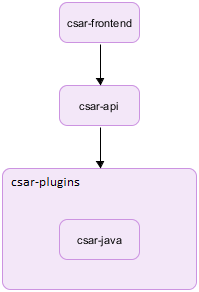
\includegraphics{figure-1}
\end{figure}

The frontend receives user input and directs them to the `csar-api', which in turn interacts with its plugins to complete the user's task.

The `csar-api' defines the csar query, csar plugins (using Java's ServiceLoader class), various interfaces (for parsing, searching, and refactoring), and various utilities (for plugins and otherwise).
It does not specify language-specific implementation details.

The language-specific details are specified in plugins.
These behaviours are: code parsing, post-processing, searching, and refactoring.

\subsubsection{csar-cli}
% TODO write

\subsubsection{csar-api}
% TODO write

\subsubsection{Plugins}
Plugins must adhere to the following rules:
\begin{itemize}
  \item They are not executed concurrently, but interleaving during the same step of csar process may occur, i.e. all plugins may be told to parse one by one, and then to post-process one by one, and so forth.
  \item They will have unrestricted access to the host machine.
  \item All plugins have access to all project files, thus it is possible for two plugins to modify the same file.
\end{itemize}

To use a plugin with csar the following must be done:
\begin{itemize}
  \item Place the project JAR in the the same directory as csar (which should be the current working directory).
  If you place it in any other directory, including a sub-directory, csar is not obliged to detect it but it may at its own discretion.
  \item Run the csar front-end jar, then `csar-api' should automatically detect and delegate tasks to the plugin.
\end{itemize}

\subsubsection{csar-java}
% TODO write

% Implementation
\section{Implementation}
This section describes csar's implementation details, that is, the exact algorithms and ideas of interest used.

\subsection{Csar query}
The implemented version of the Csar Query language is a superset of v1.2.0.
Its `expr' rule is very lenient, this is because the definition of an expression depends on a target programming language. 
This is intended to be parsed further at a language-specific level.
The grammar should explicitly allow the escaping of single quote in the comment rules, but it works anyway.
`REGEXP` rules can be swallowed by other rules, we must make sure its used strictly for regex characters and not string literals.

Some example queries built using the language are specified below:
\begin{itemize}
  \item `SELECT method:use:print' - will find method calls with the identifier `print'.
  \item `SELECT method:use:REGEXP(print*)' - will find method calls starting the identifier `print'.
  \item `SELECT method:def:static final print(1)' - will find method definitions which are static and final, with the identifier `print' and one argument.
  \item `SELECT method:def:print(String)' - will find method definitions with the identifier `print' and one `String' argument.
  \item `SELECT method:def:print REFACTOR rename:anotherPrint' will find methods with the identifier `print', and then rename them and their corresponding method calls to `anotherPrint'.
  \item `SELECT method:def:print REFACTOR changeparam:String s, String s1' - will find methods with the identifier `print', and then rename them and their corresponding method calls to `anotherPrint'.
\end{itemize}

\subsection{Ignore files}
Ignore files is split into two parts: creating ignore rules, and applying them.
Rules are split into two categories: a flexible rule (may be a file or directory), and a rule (is either a file or a directory).
Rules are specified in a git rules-like format.

Firstly, creating ignore rules can be done by reading a file containing rules, or taking as argument a `String' containing rules.
When these rules are read, they are converted into a specialized regular expression called a `PathMatcher', which is then used to check if a file is matched by a rule.
This is typically done by iterating over a list of rules, and checking if any of them match an argument file.

This may have an issue where it does not fully support ignore files.

\subsubsection{Plugins}
To create a plugin for csar the following must be done:
\begin{itemize}
  \item Create a new project targeting the JVM which depends on: `csar-api'.
  \item Create a class which implements `CsarPlugin' from `csar-api'.
  This must have a public 0-arguments constructor, and must implement the behaviour defined by the interface: parsing, post-processing, searching, and refactoring.
  Your implementation should support adding and removing error listeners as specified by the interface, and delegating the appropriate errors to them.
  The skeleton of this class can be seen in the appendices (see \ref{apx:SkeletonCsarPluginImplementation}).
  \item Define a resource for the JAR, which should be in the `META-INF/services' folder.
  The file's name should be `org.qmul.csar.plugin.CsarPlugin' and its content the fully qualified name of your plugin.
  In the case of the appendix implementation this would be `org.qmul.csar.CsarJavaPlugin'.
  \item Compile the project into a JAR.
\end{itemize}

Plugins are loaded at runtime using the `CsarPluginLoader' singleton class, which utilises a `ClassLoader' to find the JARs and `ServiceLoader' to load the plugin classes.

\subsection{Parsing}
% TODO write

\subsubsection{Parsing Java Code}
% TODO write

\subsection{Post-processing}
% TODO write

\subsubsection{Overridden methods resolver}
% TODO write

\subsubsection{Method use resolver}
% TODO write

\subsubsection{Qualified name resolver}
% TODO write

\subsubsection{Type hierarchy resolver}
% TODO write

\subsubsection{Expression type resolver}
% TODO write

\subsection{Searching}
% TODO write

\subsubsection{Java implementation}
% TODO write

\subsection{Refactoring}
% TODO write

\subsubsection{Java implementation}
% TODO write

\subsection{Code references}
\label{sec:CodeReferences}
csar has reused some code, or ideas from external sources within its code. They are listed below:
\begin{itemize}
  \item Ignore files syntax - \url{https://git-scm.com/docs/gitignore} and \url{https://github.com/EE/gitignore-to-glob/blob/master/lib/gitignore-to-glob.js}
  \item Test cases for ignore files - \url{https://www.atlassian.com/git/tutorials/gitignore}
  \item Git repository integration - \url{https://git-scm.com/docs/git-ls-files}
  \item Mercurial repository integration - \url{https://kapeli.com/cheat_sheets/Mercurial.docset/Contents/Resources/Documents/index#//dash_ref/Category/Work%20Status/1}
  \item Subversion repository integration - \url{http://svnbook.red-bean.com/en/1.7/svn.ref.svn.c.status.html}
  \item Java 8 ANTLR Grammar - \href{https://github.com/antlr/grammars-v4/blob/02711067f82bed8e0c8dfd25e80f4f8ae2472abd/java8-pt/JavaLexer.g4}{Java 8 Lexer}, \href{https://github.com/antlr/grammars-v4/blob/02711067f82bed8e0c8dfd25e80f4f8ae2472abd/java8-pt/JavaParser.g4}{Java 8 Parser}, \href{https://github.com/antlr/grammars-v4/blob/02711067f82bed8e0c8dfd25e80f4f8ae2472abd/_grammar-test/src/test/java/TestJava8pt.java}{Java 8 Test} and \href{https://github.com/antlr/grammars-v4/blob/02711067f82bed8e0c8dfd25e80f4f8ae2472abd/java8-pt/examples/AllInOne8.java}{Java 8 Test Input}
  \item `JAVA\_LETTER' rule in `CsarLexer' - \url{https://github.com/antlr/grammars-v4/blob/master/java8/Java8.g4}
  Hence, I have not written the Java 8 lexer, parser, testing code, nor the testing resources.
  \item Using JCommander parameters in `CsarContext' - \url{http://jcommander.org/}
  \item Counting substring occurrence in a String - \url{https://stackoverflow.com/a/767910}
\end{itemize}

\subsection{Gradle references}
Gradle is configured through scripts, the following references were used to help create them. They are listed below:

\begin{itemize}
  \item ANTLR process settings in `build.gradle' - \url{https://docs.gradle.org/4.0.1/userguide/antlr\_plugin.html\#sec:controlling\_the\_antlr\_generator\_process}
  \item JaCoCo in `build.gradle' - \url{http://www.jworks.nl/2013/06/03/jacoco-code-coverage-with-gradle/}
\end{itemize}

% Testing
\section{Testing}
This section describes the two main testing mechanisms I used, which are unit testing and manual testing.
Some of csar was developed in a test-driven manner, that is, I wrote the tests corresponding to features first and then wrote code to make them work.

In the unit testing section there will be mentions of statistics, some are generated by my IDE (IntelliJ IDEA) and the rest by the JaCoCo (Java Code Coverage) Gradle plugin.
These statistics may be misleading in some instances, e.g. they account for the testing of `toString()' implementations which may not be interesting in most scenarios.

Notation: Language constructs will be written within quotes.
Method names lead with `\#', e.g. `\#helloWorld' is a method called `helloWorld', similarly `Helper\#print' is a method called `print' in a type called `Helper'.
If there is no method, then the quotation may be representing a package if all in lowercase, or otherwise a Class.

\subsection{Unit testing}
The following will describe the unit tests present in csar modules.

\subsection{csar-cli}
csar-cli heavily depends on csar-api and doesn't provide a lot behaviour of its own, hence it is not tested with high coverage.

The only unit tests are on the `ResultFormatter' subclasses `JsonResultFormatter' and `PlainTextResultFormatter', which format results as Strings.
Each is tested for its output given an empty list of results, a list of one valid result, and a list of two valid results.

This results in six tests which are all successful, achieving 94\% coverage on the `org.qmul.csar.result.formatter' package.

\subsection{csar-api}
csar-api consists mostly of interfaces, hence it is not tested with high coverage.

Firstly, ignore files (`com.purecs.ignorefiles') are tested for file and directory rule parsing, and then for applying these rules on files.
The specific test cases were largely taken from the internet (see \ref{sec:CodeReferences}).

Secondly, the `DefaultProjectCodeParser' is tested for invalid constructor arguments.
Its test cases are: providing an invalid number of threads - a negative number or zero, providing a `null' iterator, and providing a `null' CodeParserFactory.

Thirdly, `ContainsQuery\#validate' is tested.
Its test cases include: a descriptor, the not operator followed by a descriptor, two consecutive operators, two consecutive descriptors, leading or ending with an invalid operator, and combinations of the aforementioned.

Then, `CsarQueryFactory\#parse' is tested.
Its test cases include: empty query, queries with a from clause, queries with refactor clause, queries with a contains clause, and syntactically invalid queries.

Then, `FilterableIterator' is tested.
Its test cases include: creating it with a list of paths and a filter, and then consuming its `\#hasNext' and `\#next' methods.

Then, `NamedThreadFactory' is tested.
Its test cases include: its creation, and verifying the names of the first two threads it creates.
This is done for two valid naming formats, and providing `null' as the naming format.

Finally, `StringUtils' is tested.
Its `\#indentation' is tested in two cases: a positive integer, and zero.
Its `\#fileNameWithoutExtension' is tested in three cases: a directory input, a file name with an extension, and a file name without an extension.
Its `\#count' method's test cases include: counting the empty string, counting within the empty string, and testing case-sensitivity in the counting.

This results in 47 tests which are all successful, achieving 55\% coverage in this module.
This coverage figure is less than expected because it includes coverage for the csar query parser-generator code, which is auto-generated by ANTLR.
This code is very long and not thoroughly tested because not all of its functionality is used yet.

\subsection{csar-java}
Firstly, the ANTLR generated Java 8 parser-generator is tested.
Its test cases are taken from ANTLR's repository (see \ref{sec:CodeReferences}) and span 36 input classes.

Secondly, the `JavaCodeParser' is tested.
Its test cases span thirteen input classes.

Thirdly, `OverriddenMethodsResolver' is tested.
Its test cases include resolving: methods with identical signatures, methods with arguments with dimension (i.e. arrays), methods with generic argument types, methods which have subtypes in their arguments, regular overridden methods and regular non-overridden methods.

Then, `MethodUseResolver' is tested.
Its test cases include method calls: in the current class, in the current class which is recursive, in the current class which is static, on a variable, using the `this' and `super' keywords, on a method, with subtype arguments, on a fully qualified name which is static, and on the parent instance from within an inner class.

Then, `TypeHierarchyResolver' is tested.
Its test cases include sub-typing of types: in the same package, which are enums, in multiple-inheritance uses, which are inner types, which are the super class, and in the default package.
Furthermore, the Java property that all classes must have `java.lang.Object' as their root superclass is tested for types which are: top-level, inner classes, and in the default package.
Finally, the type hierarchy of Java primitive types are tested \autocite{javadocsnumber}.

Then, `TypeHelper' is tested.
Its `\#normalizeVarArgs', `\#removeDimensions', and `\#dimensions' are tested in multiple cases including: a type, a fully qualified type, a type array, a type array with varargs, and a type with varargs.
Its `\#removeGenericArgument' is tested in five cases including: a type, a type array, a type with a generic argument, a type with two generic arguments, and a type array with a generic argument which is an array.
Its `\#resolveGenericTypes' is tested in two cases including: a type with two generic arguments, and one which has a generic argument extending another generic argument.
Its `\#identifierOfGenericTypeParameter' is tested in three cases including: a generic argument, a generic argument which extends a type, and a generic argument array which extends a generic argument array array.
Its `\#applyTypeParameter' is tested in 18 cases including: types without generic arguments, types with a single generic argument, types with multiple generic arguments, types with generic argument arrays, and types with a generic argument with a generic argument.
Its `\#eraseBoundsOnTypeParameter' is tested in four cases including: a generic argument, a generic argument extending another generic argument, and anonymous types extending generic types.
Its `\#eraseBounds' is tested in five cases including: a class without generic arguments, a class with generic arguments, and a class with multiple generic arguments some of which extend other classes.
Its `\#extractGenericArgument' is tested in four ways including: a type without generic arguments, a type with generic arguments, and a type array with a generic argument array.

Then, `ChangeParametersRefactorer\#setLines' is tested for four test cases, in which we set the contents of: multiple lines such that lines are collapsed, a blank line, a single line, and multiple lines.

Then, `JavaCodeSearcher' is tested.
Its test case includes three classes: A, B which extends A, and C which has a constructor calling a method on A, and a static constructor calling a method on B.
It has five test cases which are the following queries searching for method usages and definitions: ``SELECT method:use:print'', ``SELECT method:use:print(String)'', and ``SELECT method:def:print'', ``SELECT method:def:print(String)'', and ``SELECT method:def:print(1)''.

Finally, `JavaCodeRefactorer' is tested.
Each of its test case correspond to a collection of three unique classes: A, B, and C, which interact with each other in various ways.
It has four test cases which are the following queries refactoring methods: ``SELECT method:def:print REFACTOR rename:anotherPrint'', ``SELECT method:def:print REFACTOR changeparam:int a'', ``SELECT method:def:print REFACTOR changeparam:String s, String s1'', ``SELECT method:def:print REFACTOR changeparam:int a, int b, int c'', and ``SELECT method:def:print REFACTOR changeparam:int a, int b, int c''.

This results in 87 tests which are all successful, achieving 65\% coverage in this module.
This coverage figure is less than expected because it includes coverage for the Java 8 parser-generator code.

\subsection{Manual testing}
% TODO write

% Analysis
\section{Analysis}
This section will evaluate the achievements of the project, the author, and future work which ties in with this project.

\subsection{Project's achievements}
Firstly, I will examine csar's primary requirements (see \ref{sec:PrimaryRequirements}).

Primary requirement 1 was implemented. 

Primary requirement 2 was implemented, however it does have some issues (see \ref{sec:DesignCsarQuery}).

Primary requirement 3 was partially implemented.
I used a pre-written ANTLR grammar which I modified. 
It contains a minor defect which is that it doesn't handle source files with more than one top-level class.
The grammar is not very strict for efficiency purposes.

Primary requirement 4 was partially implemented, support for the `CONTAINS' clause in the csar query is not implemented.
Furthermore, the `toPseudoCode()' method is used to generate code fragments to display in the output results.
This method is not tested for every implementation of it, which means some of the code fragments may be partially incorrect.

Primary requirement 5 was implemented.

Primary requirement 6 and 7 were implemented, however I think refactoring could benefit from more testing.
The refactoring interfaces could also be improved, there are some unused methods, and messy code.

Primary requirement 8 was implemented.

Primary requirement 9 was partially implemented. The first issue is that method references are not handled.
The second issue is that csar does not support external libraries (i.e. it does not recognize their types) - this also extends to the Java 8 standard library.
This is because without efficient, and complete indexing (also known as caching) capabilities this would slow down csar too much.

Secondly, I will examine csar's secondary requirements (see \ref{sec:SecondaryRequirements}).

Secondary requirement `Indexing parsed project source code' was not implemented.
This is because it would require clarification on where csar's supporting binaries and caches should reside, which would imply that an installer would need to be created.
It would also require us to index post-processing, searching, and refactoring results to fully exploit indexing.
Some of these are very complicated.
Suppose we wanted to index the project's type hierarchy, we would need to figure out how the changed files change the type hierarchy without calculating it all from scratch.

Secondary requirement `Supporting Mercurial (hg)/Subversion (svn) repositories' was implemented, however it was not thoroughly tested because I am not proficient enough in Subversion nor Mercurial.

Secondary requirement `IntelliJ IDEA integration' was not implemented.
I never intended to implement it because I do not consider it very important, and IntelliJ is updated too often for me to have enough time to keep it updated.
It was included in the requirements so that I could outline how a potential implementation of it would work.

Secondary requirement `Ignore files' was implemented.
It may however not fully support trailing spaces in file names.

Thirdly, I will examine csar's non-functional requirements (see \ref{sec:NonFunctionalRequirements}).

Requirement 1 was implemented.
For the most part I followed the formal Javadocs style, I strayed from it occasionally because I find it repetitive for certain kinds of documentation (e.g. getters, setters, and constructors).

Non-functional requirement 2 was partially implemented.
Some of the algorithms are not polynomial time, but the use of caching has helped alleviate such concerns where appropriate.
The most time consuming tasks in csar are: code parsing, and post-processing.

Non-functional requirement 3 was implemented, however there is room for improvement.
Some of the design could benefit from being reworked, now that my knowledge of this area is greater.

Non-functional requirement 4 was implemented.

Non-functional requirement 5 will be implemented once my project is graded, to prevent self-plagiarism.

Non-functional requirement 6 was implemented, csar was written using Java 8.

Non-functional requirement 7 was partially implemented.
The biggest issue of note is that interface mocking is not used enough, leading to multiple tests relying on each other working to work themselves.
This might make detecting bugs harder than otherwise.
JaCoCO has some defects which mean its reports are not very accurate.
For example, it counts setters and getters in its coverage statistics.

Non-functional requirement 8 was partially implemented.
The only major operations which are not multi-threaded are the following post-processors: `QualifiedNameResolver', `TypeHierarchyResolver', `MethodQualifiedTypeResolver', `MethodUseResolver', and `MethodCallTypeInstanceResolver'.

Non-functional requirement 9 was implemented.

\subsection{Author's achievements}
This was a one of the biggest, most ambitious, and longest lasting projects I have worked on.
It thoroughly tested my resolve, discipline, time management, and programming ability due to its immense complexity.

This was the first time I used Gradle, and deployed a build tool in a multi-module project.
It was also the first time I used the ANTLR, JCommander, and Mockito libraries.
It was also the first time I used TeX, and wrote a language grammar from scratch (csar query).

It contributed greatly to my understanding of multi-threading, Subversion/Mercurial, Java 8 lambdas, Java 8 syntax intricacies, and the Java ServiceLoader (for the plugin system).

It also led to me making my first open-source contribution on a big project.
It was the first time I had to discuss my ideas and seek approval from developers I had no prior relationship with in order to get my changes accepted.
I also had the pleasure of working with highly esteemed developers, including Cedric Beust on JCommander, who created the Android Gmail application.
This was followed up with numerous commits on the ANTLR grammars-v4, and JCommander repositories (see \ref{apx:OpenSourceContributions}).

\subsection{Future work}
A wider range of searching and refactoring tools should be evaluated, to guide future development of csar and focus efforts on the most important features.

The plugin system should be improved by potentially allowing language-specific query languages.
Furthermore, it could be enhanced by setting strict permissions on plugins to prevent unexpected or malicious behaviour.
For example, perhaps plugins cannot access or modify system files, or access the internet.

It would be useful to rewrite Csar Query as part of an elaborate research project.
Then, csar could be reimplemented in full, with changes focused on csar-java, in an attempt to ensure it is bug-free, and theoretically sound.

This could be followed up with an implementation for a dynamically-typed programming language such as Python \autocite{learningpython5thed}, so that future developers can use it to develop support for similar languages.

There are plenty of refactoring operations that could be supported, such as: move code, detect duplicate code, change signature (change parameters is a subset of this), convert anonymous to inner, encapsulate fields, inline, replace constructor with builder or factory method, etc. \autocite{intellijidearefactoring}.

It would also be optimal for the refactoring to maintain the current conventions of the code file being edited.

% Bibliography
\section{Bibliography}
\printbibliography[heading=none]

% Appendices
\section{Appendices}

% Appendix 1: Open-source contributions
\subsection{Open-source contributions}
\label{apx:OpenSourceContributions}
Repository: \href{https://github.com/antlr/grammars-v4}{antlr/grammars-v4}
\begin{itemize}
  \item ``Disallow local enums/annotations in Java8PT grammar'' (\href{https://github.com/antlr/grammars-v4/pull/886}{Pull Request \#886} and \href{https://github.com/antlr/grammars-v4/pull/887}{Pull Request \#887})
  \item ``Allow method reference leading with `this` in Java8PT grammar + minor reformatting'' (\href{https://github.com/antlr/grammars-v4/pull/898}{Pull Request \#898})
  \item ``Improve Java8PT methodReference rule'' (\href{https://github.com/antlr/grammars-v4/pull/901}{Pull Request \#901})
\end{itemize}

Repository: \href{https://github.com/cbeust/jcommander}{cbeust/JCommander}
\begin{itemize}
  \item ``Fix misc.xml'' (\href{https://github.com/cbeust/jcommander/pull/407}{Pull Request \#407})
  \item ``Flexible usage formatting'' (\href{https://github.com/cbeust/jcommander/pull/408}{Pull Request \#408})
  \item ``Java 7 compliance'' (\href{https://github.com/cbeust/jcommander/pull/409}{Pull Request \#409})
  \item ``Fix locale-related issues in usage formatter tests'' (\href{https://github.com/cbeust/jcommander/pull/410}{Pull Request \#410})
  \item ``Add documentation for usage formatter'' (\href{https://github.com/cbeust/jcommander/pull/411}{Pull Request \#411})
  \item ``Update changelog'' (\href{https://github.com/cbeust/jcommander/pull/419}{Pull Request \#419})
\end{itemize}

% Appendix 2: Skeleton of a CsarPlugin Implementation
\subsection{Skeleton of a CsarPlugin Implementation}
\label{apx:SkeletonCsarPluginImplementation}

\begin{lstlisting}[language=Java]
package org.qmul.csar.CsarJavaPlugin;

// imports...

/**
  * The Java language csar plugin.
  */
public class CsarJavaPlugin implements CsarPlugin {

  @Override
  public void parse(Path projectDirectory, boolean narrowSearch, Path ignoreFile, int threadCount) {
    // parse code...
  }

  @Override
  public void postprocess(int threadCount) {
    // post-process code...
  }

  @Override
  public List<Result> search(CsarQuery csarQuery, int threadCount) {
    // search code...
  }

  @override
  public List<Result> refactor(CsarQuery csarQuery, List<Result> searchResults, int threadCount) {
    // refactor code
  }

  @Override
  public void addErrorListener(CsarErrorListener errorListener) {
    // add the error listener...
  }

  @Override
  public void addErrorListener(CsarErrorListener errorListener) {
    // add the error listener...
  }

  @Override
  public void removeErrorListener(CsarErrorListener errorListener) {
    // remove the error listener...
  }
}
\end{lstlisting}

% Appendix 3: Csar Query Language v1.2.0
\subsection{Csar Query Language v1.2.0}
\label{apx:CsarQueryLanguagev120}

\begin{lstlisting}
/**
 * Lexer
 */
lexer grammar CsarLexer;

/*
 * The lexer rules have been omitted for brevity, because their names are very good indicators
 * of exactly what they are. Each rule represents a literal or range of literals.
 * You can find the full grammar in the `design-docs/query-language' folder within the project.
 */

// Language elements
IDENTIFIER_NAME: JAVA_LETTER (JAVA_LETTER | DIGIT)*;
NUMBER: DIGIT+;

// Fall-back rule
CATCH_ALL: (.)+?;

// Fragments
fragment TEXT: [a-zA-Z];
fragment DIGIT: [0-9];

// The following rule is taken from: https://github.com/antlr/grammars-v4/blob/master/java8/Java8.g4
fragment JAVA_LETTER
    :   TEXT | [$_] // these are the "java letters" below 0x7F
    |   // covers all characters above 0x7F which are not a surrogate
        ~[\u0000-\u007F\uD800-\uDBFF]
        {Character.isJavaIdentifierStart(_input.LA(-1))}?
    |	// covers UTF-16 surrogate pairs encodings for U+10000 to U+10FFFF
        [\uD800-\uDBFF] [\uDC00-\uDFFF]
        {Character.isJavaIdentifierStart(Character.toCodePoint((char)_input.LA(-2), (char)_input.LA(-1)))}?
    ;

/**
 * Parser
 */
parser grammar CsarParser;

// Csar query (top-level)
csarQuery: (SELECT SPACE)? statementDescriptor (SPACE containsQuery)? (SPACE fromQuery)? (SPACE refactorQuery)? EOF;
containsQuery: CONTAINS SPACE (NOT SPACE)? statementDescriptor containsQueryRest*;
containsQueryRest: SPACE (AND | OR) SPACE (NOT SPACE)? statementDescriptor;
fromQuery: FROM SPACE typeList; // types to search within
refactorQuery: REFACTOR SPACE refactorDescriptor;

statementDescriptor: clazz | method | variable | conditional | comment;
refactorDescriptor: rename | changeParameters;

// Class
clazz: (CLASS_NV | CLASS_V) commonModifiers classModifiers (identifierName | regexIdentifierName) superClassList?;
classModifiers: ((ABSTRACT | INTERFACE) SPACE)? (STRICTFP SPACE)? (ANONYMOUS SPACE)? (INNER SPACE)?;
superClassList: LPAREN SPACE* typeList SPACE* RPAREN;

// Method
method
    : METHOD commonModifiers (OVERRIDDEN SPACE)? (type SPACE)? (identifierName | regexIdentifierName)
     (SPACE? methodParameters)? (SPACE methodThrownExceptions)? (SPACE SUPER SPACE* superClassList)?
    ;
methodParameters: LPAREN SPACE* (NUMBER | paramTypeList | paramNamedTypeList) SPACE* RPAREN;
methodThrownExceptions: THROWS SPACE* LPAREN SPACE* typeList SPACE* RPAREN;
paramTypeList: (FINAL SPACE)? SPACE* type paramTypeListRest*;
paramTypeListRest: SPACE* COMMA (FINAL SPACE)? SPACE* type;
paramNamedTypeList: (FINAL SPACE)? type SPACE+ identifierName paramNamedTypeListRest*;
paramNamedTypeListRest: SPACE* COMMA (FINAL SPACE)? SPACE* type SPACE+ identifierName;

// Variable
variable: instanceVariable | localVariable | paramVariable;
instanceVariable: INSTANCE commonModifiers instanceVariableModifiers (type SPACE)? identifierName;
instanceVariableModifiers: ((TRANSIENT | VOLATILE) SPACE)?;
localVariable: LOCAL COLON (DEF | USE) COLON (FINAL SPACE)? (type SPACE)? identifierName;
paramVariable: PARAM COLON (DEF | USE) COLON (FINAL SPACE)? (type SPACE)? identifierName;

// Conditional
conditional: if0 | switch0 | while0 | dowhile | for0 | foreach | ternary | synchronized0;
if0: IF (LPAREN expr RPAREN)?;
switch0: SWITCH (LPAREN expr RPAREN | COLON identifierName)?;
while0: WHILE (LPAREN expr RPAREN)?;
dowhile: DOWHILE (LPAREN expr RPAREN)?;
for0: FOR;
foreach: FOREACH (COLON identifierName)?;
ternary: TERNARY;
synchronized0: SYNCHRONIZED (LPAREN expr RPAREN | COLON identifierName)?;

// Comment
comment: singleLineComment | multiLineComment;
singleLineComment: SINGLE_LINE_COMMENT (COLON S_QUOTE content S_QUOTE)?;
multiLineComment: MULTI_LINE_COMMENT (COLON JAVADOC)? (COLON S_QUOTE content S_QUOTE)?;

// Refactor
rename: RENAME COLON SPACE* identifierName;
changeParameters: CHANGE_PARAMETERS COLON SPACE* (typeList | namedTypeList);

// Helpers
commonModifiers: COLON (DEF | USE) COLON (visibilityModifier SPACE)? (STATIC SPACE)? (FINAL SPACE)?;
visibilityModifier: PUBLIC | PRIVATE | PROTECTED | PACKAGE_PRIVATE;

type: identifierName (LBRACK RBRACK)*;
typeList: type (SPACE* COMMA SPACE* type)*;
namedTypeList: type SPACE+ identifierName (SPACE* COMMA SPACE* type SPACE+ identifierName)*;
identifierName
    : IDENTIFIER_NAME | SELECT | CONTAINS | FROM | REFACTOR | DEF | USE | AND | OR | NOT | DOWHILE | TERNARY | RENAME
    | CHANGE_PARAMETERS | OVERRIDDEN | ANONYMOUS | INNER | JAVADOC | SINGLE_LINE_COMMENT | MULTI_LINE_COMMENT
    | PACKAGE_PRIVATE | INSTANCE | LOCAL | PARAM | METHOD | CLASS_NV | REGEXP
    ;
regexIdentifierName: REGEXP LPAREN (content | identifierName) RPAREN;

content
    : (SELECT | CONTAINS | FROM | REFACTOR | DEF | USE | AND | OR | NOT | CLASS_NV | CLASS_V | METHOD | INSTANCE
        | LOCAL | PARAM | IF | SWITCH | WHILE | DOWHILE | FOR | FOREACH | TERNARY | SYNCHRONIZED | SINGLE_LINE_COMMENT
        | MULTI_LINE_COMMENT | PUBLIC | PRIVATE | PROTECTED | PACKAGE_PRIVATE | STATIC | FINAL | ABSTRACT | CATCH_ALL
        | INTERFACE | STRICTFP | ANONYMOUS | INNER | SUPER | OVERRIDDEN | THROWS | RENAME | CHANGE_PARAMETERS
        | TRANSIENT | VOLATILE | JAVADOC | SPACE | COLON | COMMA | LPAREN | RPAREN | IDENTIFIER_NAME | NUMBER | S_QUOTE
        | LBRACK | RBRACK | REGEXP
      )*
    ;
expr: content;
\end{lstlisting}

\end{document}
